\documentclass{beamer}

\usepackage{wx672cjk}
\usepackage[utf8]{inputenc}
\usetheme{Madrid}
\usecolortheme{beaver}
\usepackage[labelformat=empty]{caption}
\usepackage{color}


\usepackage{hyperref}
\hypersetup{
    colorlinks=true,
    linkcolor=blue,
    filecolor=magenta,      
    urlcolor=cyan,
}
 
\urlstyle{same}
 
 
%Information to be included in the title page:
\title[\emph{ACM-ICPC}] %optional
{Programming with Funny}

\subtitle{A Problem about Happy}

\author[Qiyuan, Pu] % (optional)
{Qiyuan Pu\\ 蒲启元}



\institute[SWFU] % (optional)
{
  School of Big Data and Intelligence Engineering\\
  Southwest Forestry University
}

\date[Programming Discussion 2018] % (optional)
{Online Judge System, May 2018}

\logo{
\includegraphics[height=1.3cm]{./img/icpclogo_big.png}}

%End of title page configuration block
%------------------------------------------------------------


%------------------------------------------------------------
%The next block of commands puts the table of contents at the 
%beginning of each section and highlights the current section:

\AtBeginSection[]
{
  \begin{frame}
    \frametitle{Table of Contents}
    \tableofcontents[currentsection]
  \end{frame}
}
%------------------------------------------------------------

 
 
\begin{document}
 
%The next statement creates the title page.
\frame{\titlepage}


%---------------------------------------------------------
%This block of code is for the table of contents after
%the title page
\begin{frame}
\frametitle{Table of Contents}
\tableofcontents
\end{frame}
%---------------------------------------------------------

\section{What do you live for}
%Highlighting text
\begin{frame}
  \frametitle{What do you live for}

  \begin{figure}
    \centering
    \begin{minipage}{0.45\textwidth}
        \centering
        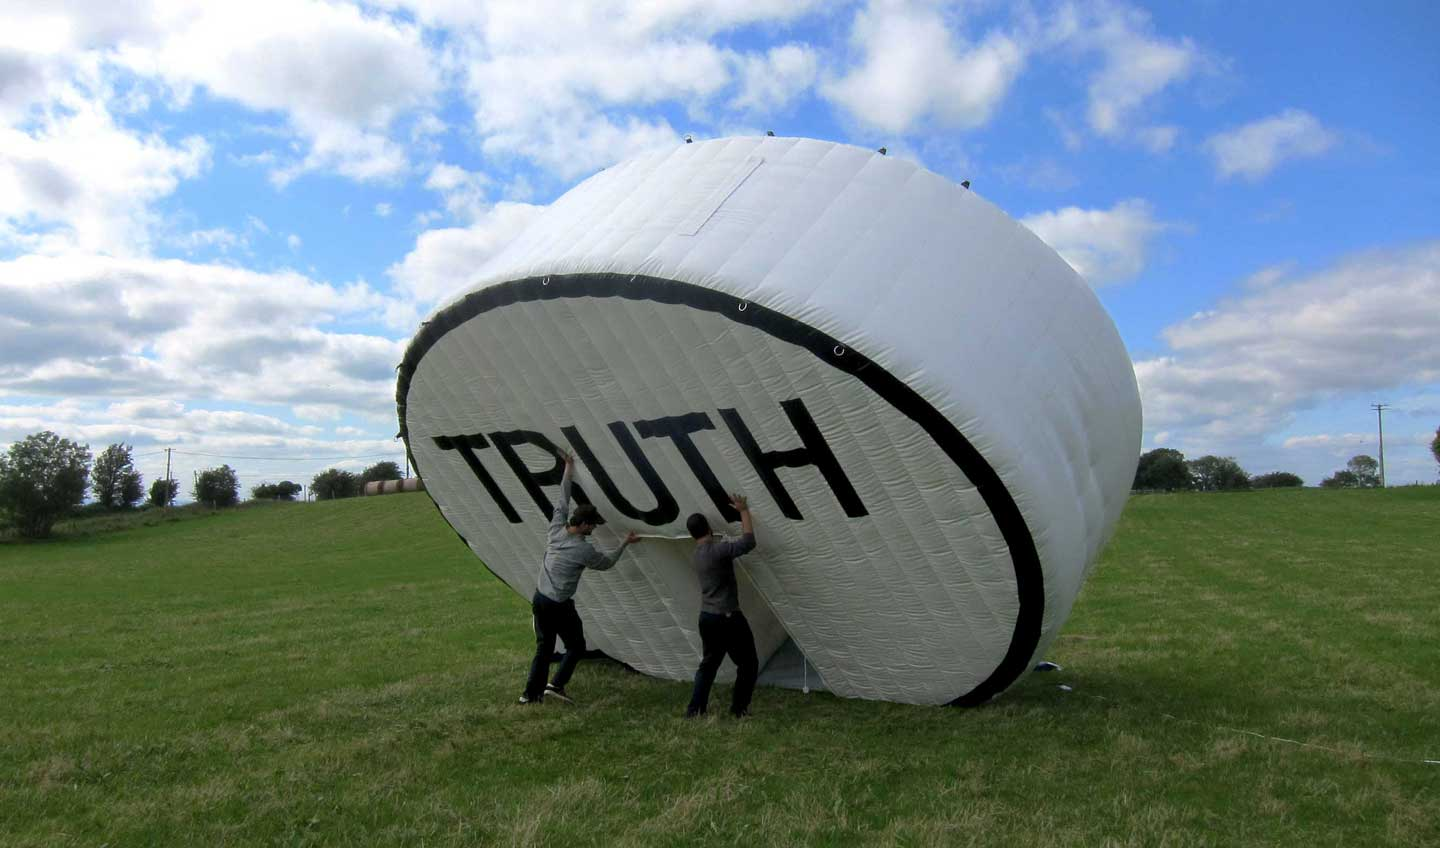
\includegraphics[width=.7\textwidth]{./img/Truth.jpg} % first figure itself
        \caption{Truth}
        \label{fig:sit-one}
    \end{minipage}\hfill
    \begin{minipage}{0.45\textwidth}
      \centering
      
\includegraphics[width=.7\textwidth]{./img/dream.jpeg} 
      \caption{Dream}
      \label{fig:sit-three}
    \end{minipage}\hfill
    \begin{minipage}{0.45\textwidth}
      \centering
      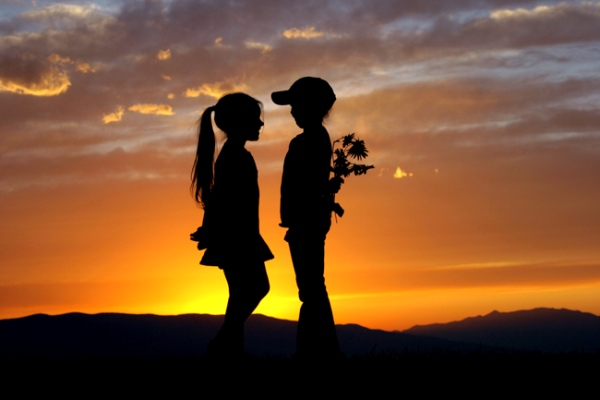
\includegraphics[width=.7\textwidth]{./img/love.jpg} 
      \caption{Love}
      \label{fig:sit-two}
    \end{minipage}\hfill
    \begin{minipage}{0.45\textwidth}
      \centering
      
\includegraphics[width=.7\textwidth]{./img/money.jpg} 
      \caption{Money}
      \label{fig:sit-four}
    \end{minipage}
    % \caption{}
    

    \textcolor{red}{What else...}
  \end{figure}
\end{frame}
  
\begin{frame}
  \frametitle{What do you live for}
  \begin{center}
    \huge {Basically, those can be reasons}
  \end{center}
  \begin{figure}
    
\includegraphics[scale=1.3]{./embed/whyHappy.pdf}
  \end{figure}
\end{frame}

\begin{frame}
  \frametitle{What do you live for}
  \begin{alertblock}{Why happy}
    \begin{enumerate}
    \item Live longer\href{http://happyproject.in/message/advantage-happy/}{(source)}
    \item More healthy\href{http://happyproject.in/message/advantage-happy/}{(source)}
    \item Marriages more succeed\href{http://happyproject.in/message/advantage-happy/}{(source)}
    \item Make more
      money\href{https://www.inc.com/rhett-power/10-reasons-why-it-is-important-create-a-happy-workplace.html}{(source)}
    \item Life should be happy, isn't it?
    \item ......
    \end{enumerate}
  \end{alertblock}

  
  \begin{center}
    \LARGE{Let's talk about one of methods to happy}
    \huge{\textcolor{red}{Programming}}
  \end{center}
  
\end{frame}


% ---------------------------------------------------------

\section{How do you think of programming}
%Highlighting text
\begin{frame}
  \frametitle{How do you think of programming}
  \begin{center}
    \huge{May you think so...}
    \begin{figure}
      
\includegraphics[scale=.38]{./img/pain11.png}
    \end{figure}
  \end{center}
\end{frame}

\begin{frame}
  \frametitle{How do you think of programming}
  \begin{center}
    \huge{Or...}
    \begin{figure}
      
\includegraphics[scale=.35]{./img/pain2.jpg}
    \end{figure}
  \end{center}
\end{frame}

\begin{frame}
  \frametitle{How do you think of programming}
  \huge{When someone calls you to running}
  \begin{center}
    \begin{figure}
      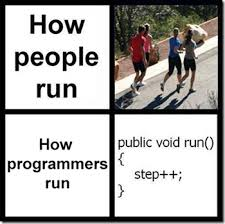
\includegraphics[scale=.35]{./img/joke1.jpeg}
    \end{figure}
  \end{center}
  
\end{frame}


\section{About Online Judge System}
%Highlighting text
\begin{frame}
\frametitle{What do you live for}

\end{frame}


\section{Some interesting problem}
%Highlighting text
\begin{frame}
\frametitle{What do you live for}

\end{frame}


\section{About ACM-ICPC}
%Highlighting text
\begin{frame}
\frametitle{What do you live for}

\end{frame}


\section{Join us}
%Highlighting text
\begin{frame}
\frametitle{What do you live for}

\end{frame}


\section{One day}
%Highlighting text
\begin{frame}
\frametitle{What do you live for}

\end{frame}


\section{Thanks}
%Highlighting text
\begin{frame}
\frametitle{What do you live for}

\end{frame}

  
 
\end{document}


%%% Local Variables:
%%% mode: latex
%%% TeX-master: t
%%% End:
